
%This is the segment that can be as long or short as needed to finish in time. Leave to end.
%Performance Analysis. Discuss impact of number of planes, size of planes, etc, with collected data. Highlight areas of improvement, engineering challenges with memory usage, reuse of buffers, reduction of memory usage by parameter tweaking, stream overlapping. Try to benchmark against other algorithms if have time, but probably won't.
\chapter{Results and Analysis}
\label{chap:analysis}
This chapter provides some example results from the finished pipeline as well as some performance analysis. The runtime of some stages of the pipeline is heavily dependent on the target scene complexity.

\section{Results}
The pipeline is tuned to look for large planar surfaces like walls, furniture, ceilings, and floors. Figure~\ref{fig:uppercorner} shows an example of a high quality segmentation result. The mesh reconstruction is visualized in the lower left corner through a virtual camera with the same intrinsic parameters as the original sensor for direct comparison. In this image, almost the entire scene is composed of planes, so the reconstruction is nearly complete.\par 
Because the Kinect is based on structured infrared light, the result is robust to varying lighting conditions. Figure~\ref{fig:uppercornerwireframelowlight} shows a darker version of the same scene with the QuadTree mesh overlaid in green.
\subsection{Successes}
\begin{figure}[!htpb]
    \centering
    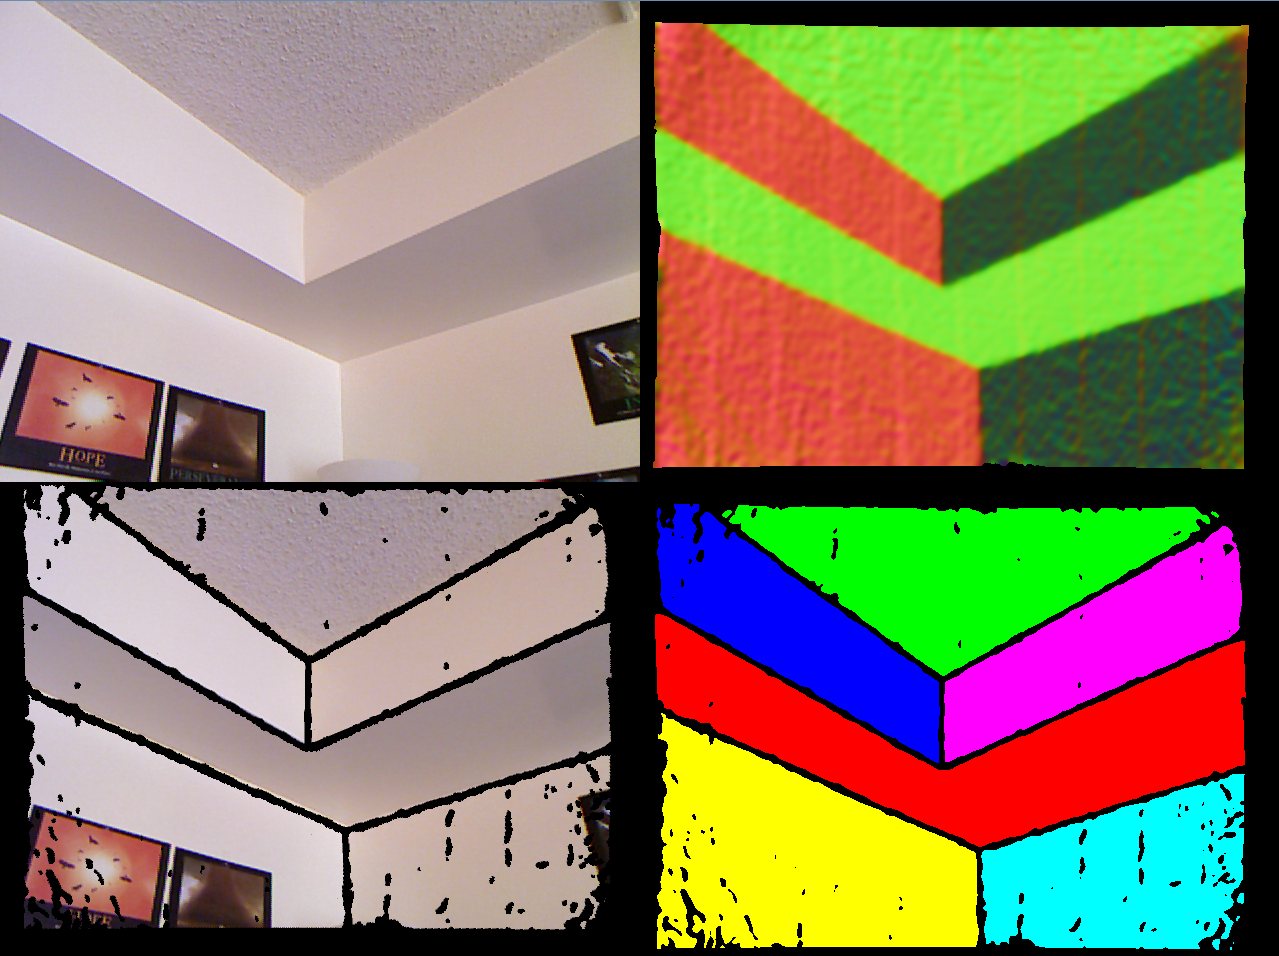
\includegraphics[width=0.8\textwidth]{UpperCornerResults.png}
    \caption{Example results of the upper corner of a room, 3 sets of 2 parallel planes detected.  Upper left) original color image. Upper right) surface normal estimates. Lower left) mesh reconstruction. Lower right) Random colorization of plane segments}
    \label{fig:uppercorner}
\end{figure}

\begin{figure}[!htpb]
    \centering
    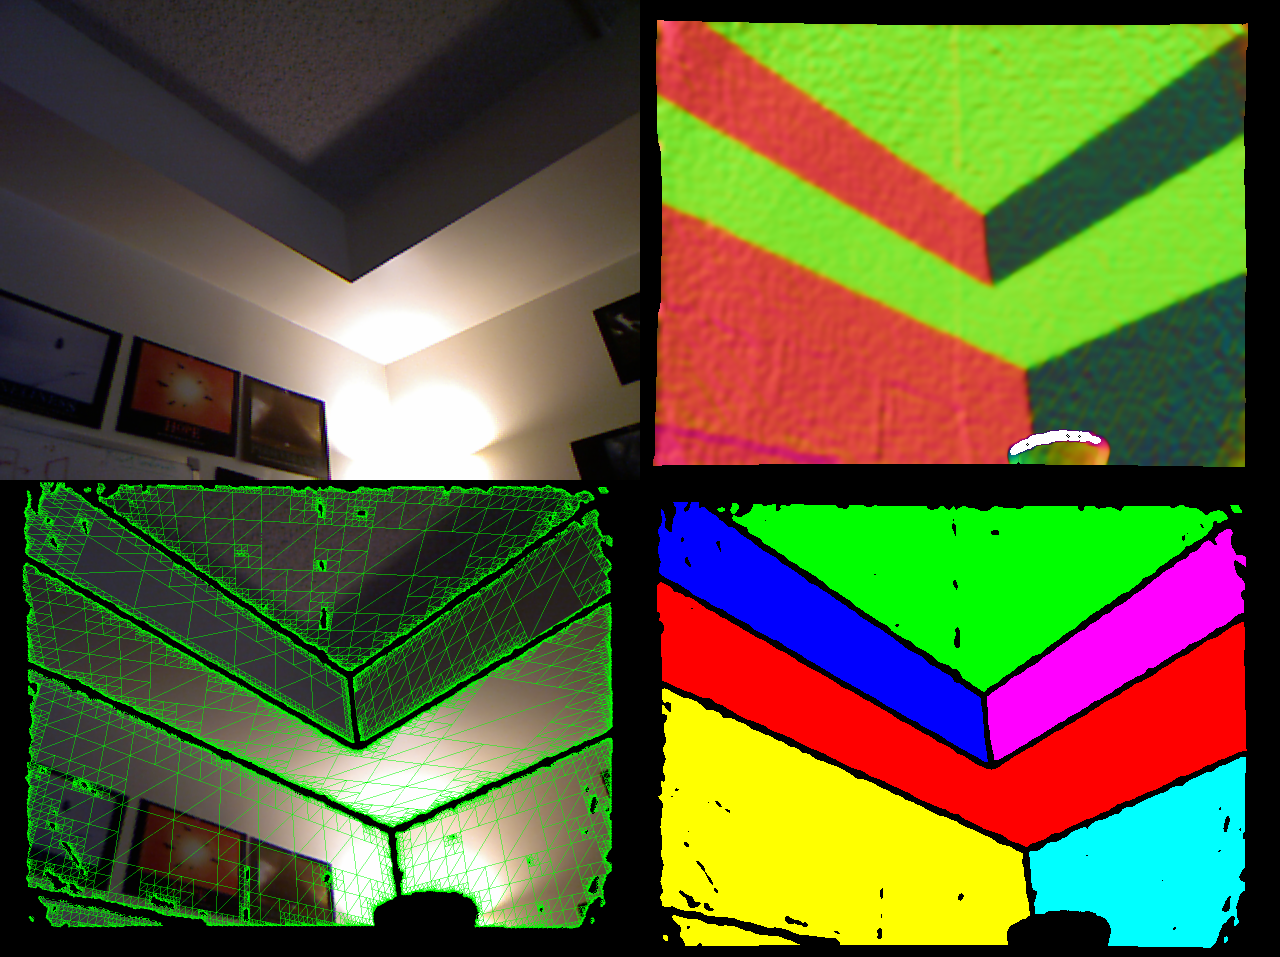
\includegraphics[width=0.8\textwidth]{UpperCornerResultsWireframe.png}
    \caption{Example results of the upper corner of a room in low light conditions with wireframe.  Upper left) original color image. Upper right) surface normal estimates. Lower left) mesh reconstruction. Lower right) Random colorization of plane segments}
    \label{fig:uppercornerwireframelowlight}
\end{figure}
As it turns out, the pipeline is very good at floor plane detection. Figure~\ref{fig:floorplane} shows a reconstruction of an empty lab floor with a tape soccer field pattern. Because the algorithm is looking for global plane solutions, the result is very robust to occlusion (Figures~\ref{fig:meshoutput} and ~\ref{fig:naoquadtree}). These images also demonstrate how adaptable the QuadTree representation is. Note that around the hole left by the robot in Figure~\ref{fig:naoquadtree} the QuadTree almost perfectly reconstructs the silhouette almost perfectly.

\begin{figure}[!htpb]
    \centering
    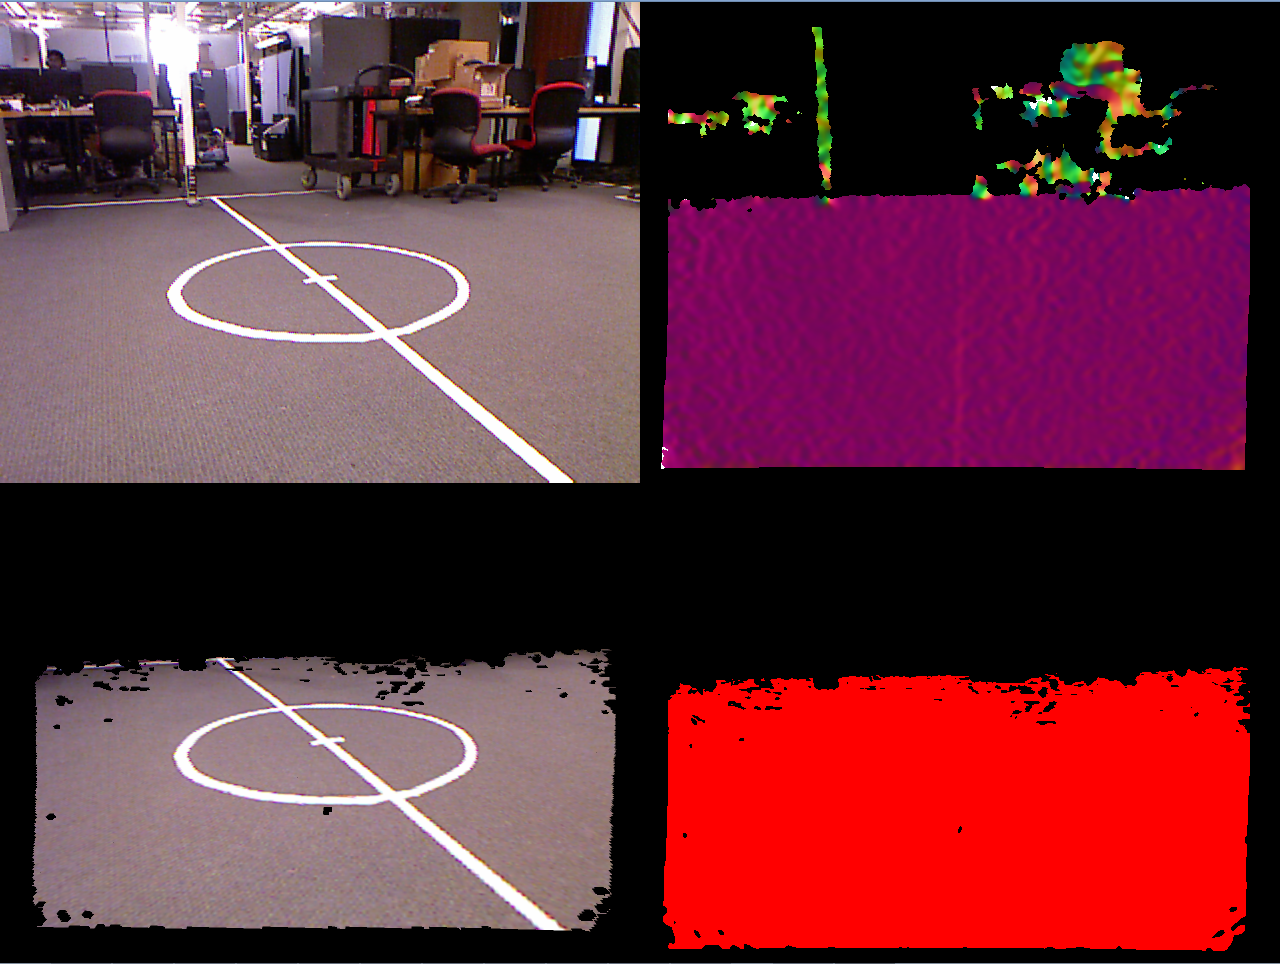
\includegraphics[width=0.8\textwidth]{EmptyGraspFieldResults.png}
    \caption{Effortless floor plane detection. Upper left) original color image. Upper right) surface normal estimates. Lower left) mesh reconstruction. Lower right) Random colorization of plane segments}
    \label{fig:floorplane}
\end{figure}


\begin{figure}[!htpb]
    \centering
    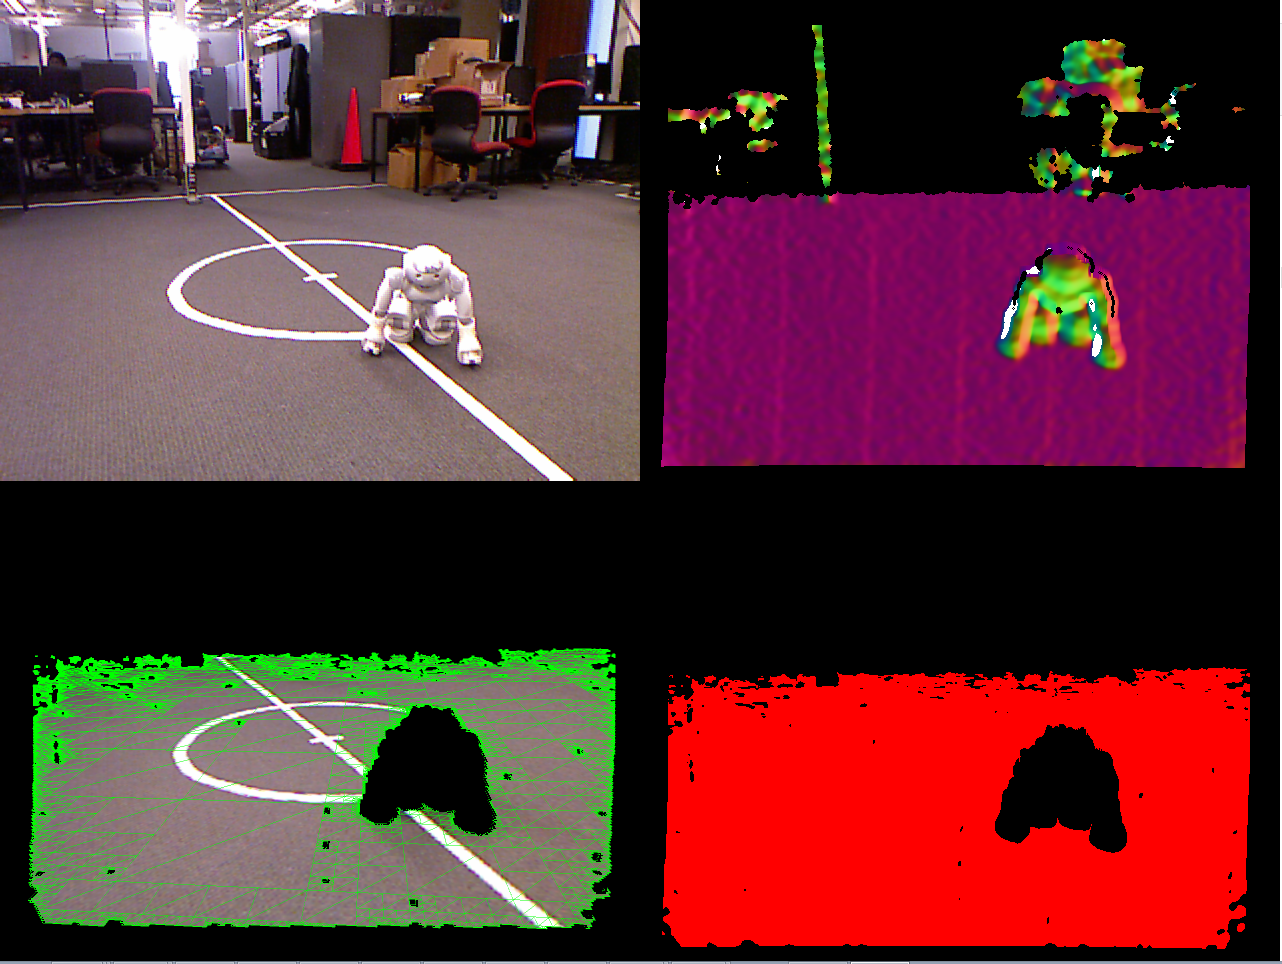
\includegraphics[width=0.8\textwidth]{NaoGraspFieldResults.png}
    \caption{Lab floor with small obstruction to demonstrate QuadTree flexibility. Upper left) original color image. Upper right) surface normal estimates. Lower left) mesh reconstruction. Lower right) Random colorization of plane segments}
    \label{fig:naoquadtree}
\end{figure}


\subsection{Failures}
However, the pipeline does have several issues an common failure cases.
\begin{figure}[!htpb]
    \centering
    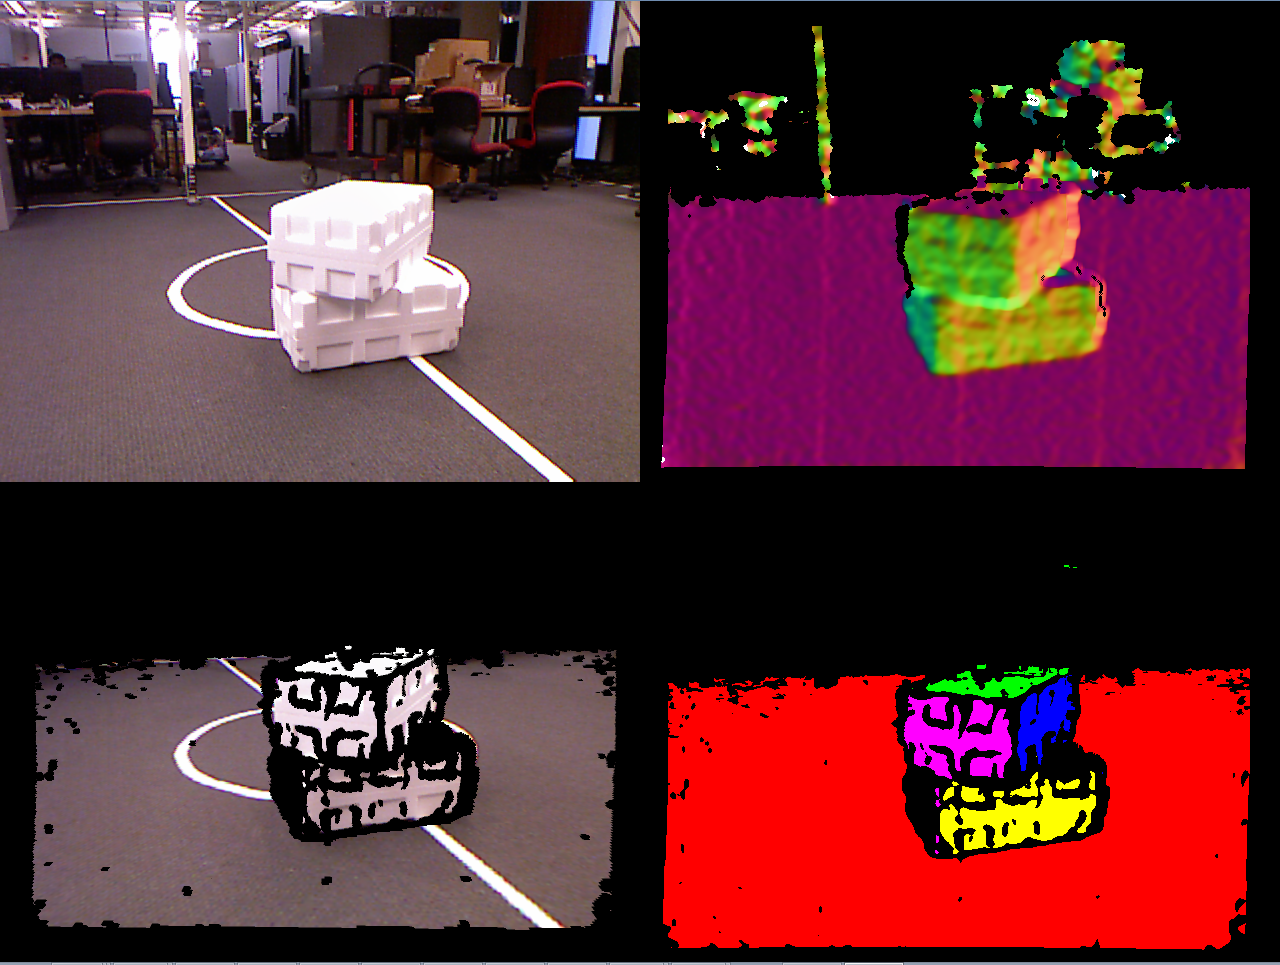
\includegraphics[width=0.8\textwidth]{FoamBoxesResults.png}
    \caption{Algorithm has difficulty with pseudo-planar surfaces. Upper left) original color image. Upper right) surface normal estimates. Lower left) mesh reconstruction. Lower right) Random colorization of plane segments}
    \label{fig:foamboxes}
\end{figure}


\begin{figure}[!htpb]
    \centering
    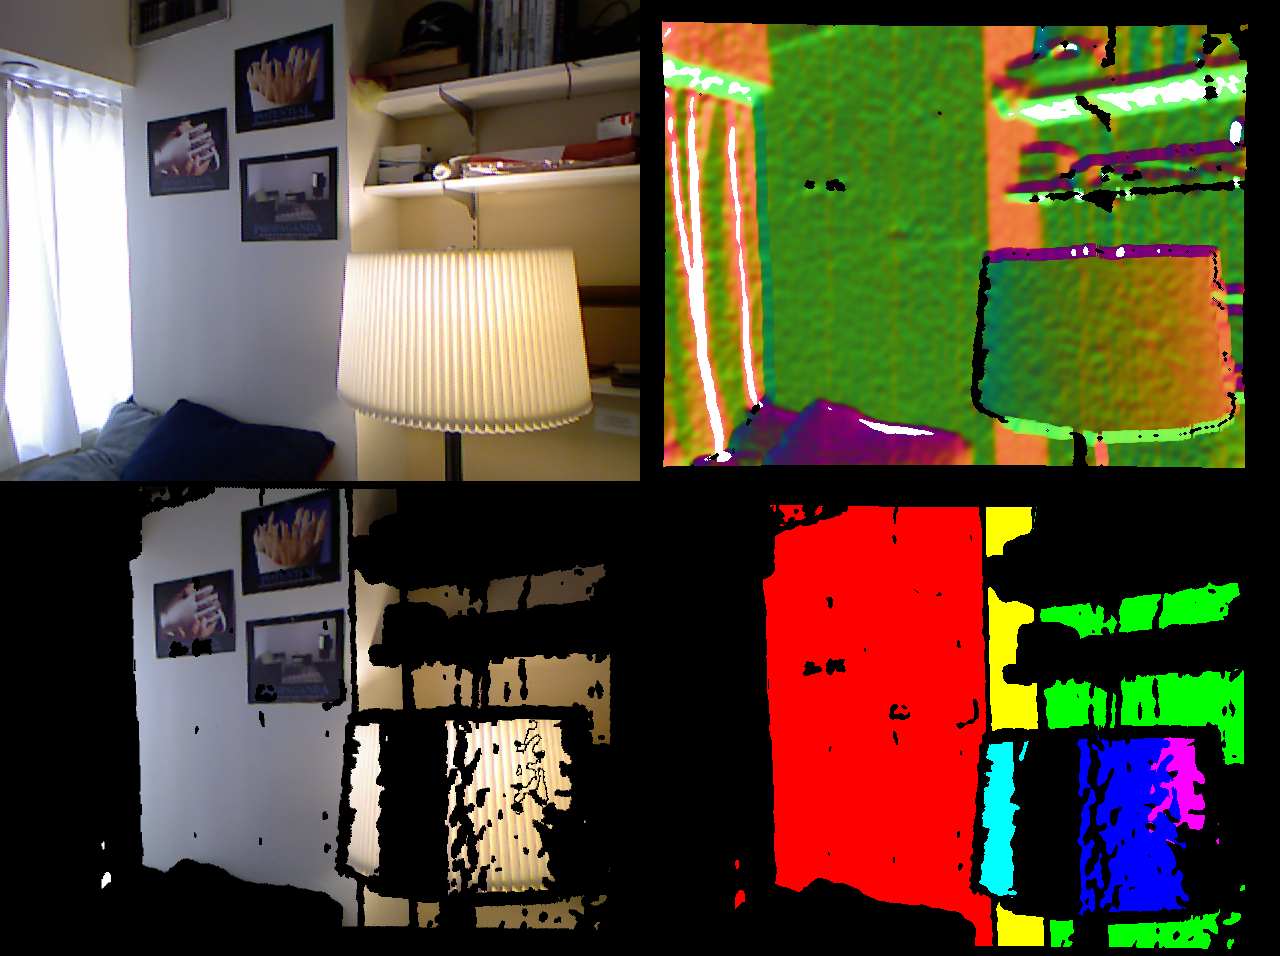
\includegraphics[width=0.8\textwidth]{LampFailureResults.png}
    \caption{Algorithm incorrectly detects large smooth curves as multiple planes. Upper left) original color image. Upper right) surface normal estimates. Lower left) mesh reconstruction. Lower right) Random colorization of plane segments}
    \label{fig:lampcurve}
\end{figure}



\begin{figure}[!htpb]
    \centering
    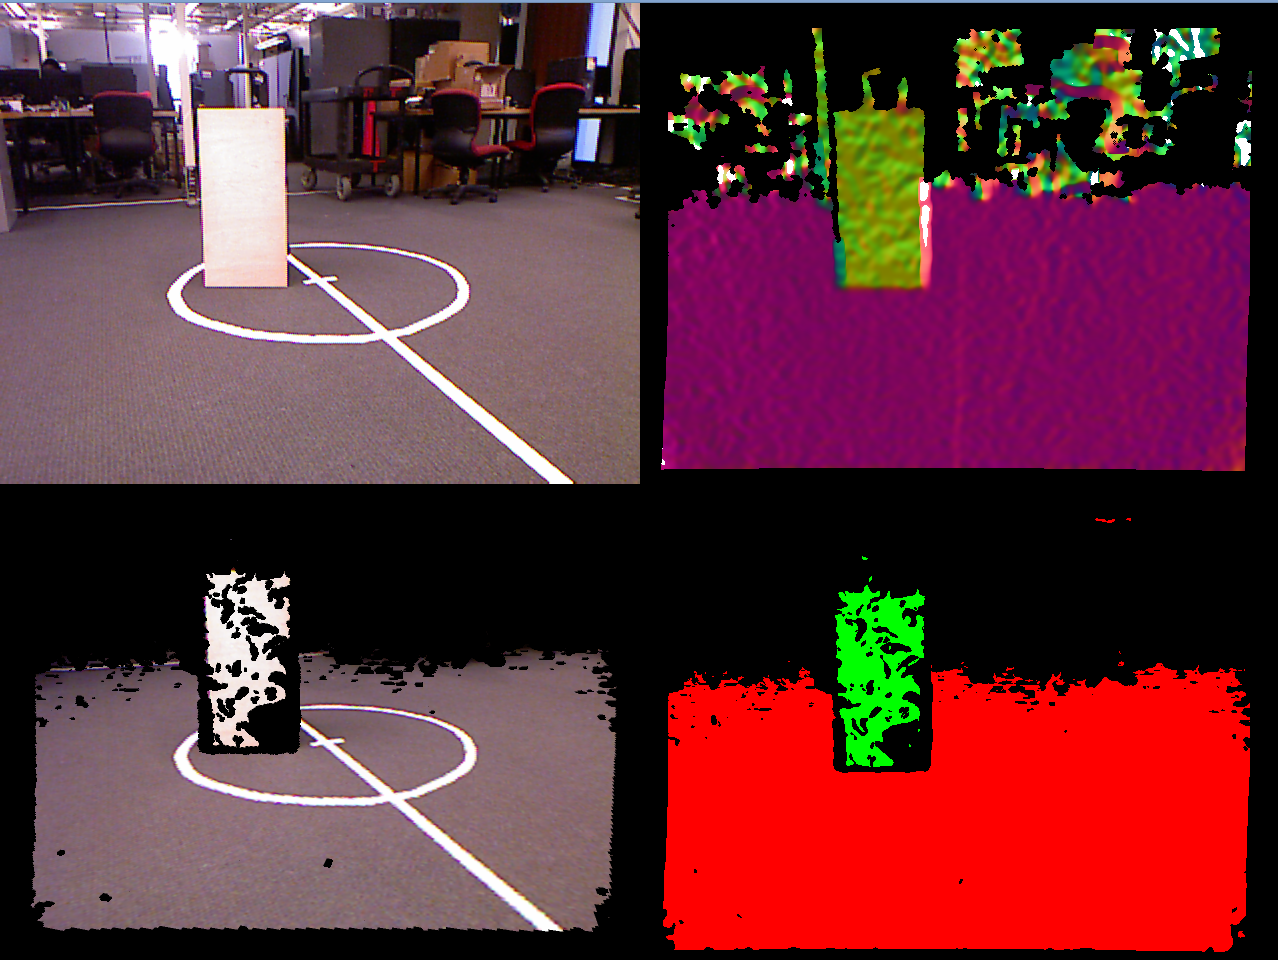
\includegraphics[width=0.8\textwidth]{BoardAndBoxResults.png}
    \caption{Fails to cleanly detect obvious plane 2.5m away. Upper left) original color image. Upper right) surface normal estimates. Lower left) mesh reconstruction. Lower right) Random colorization of plane segments}
    \label{fig:distantsmallplane}
\end{figure}




\begin{figure}[!htpb]
    \centering
    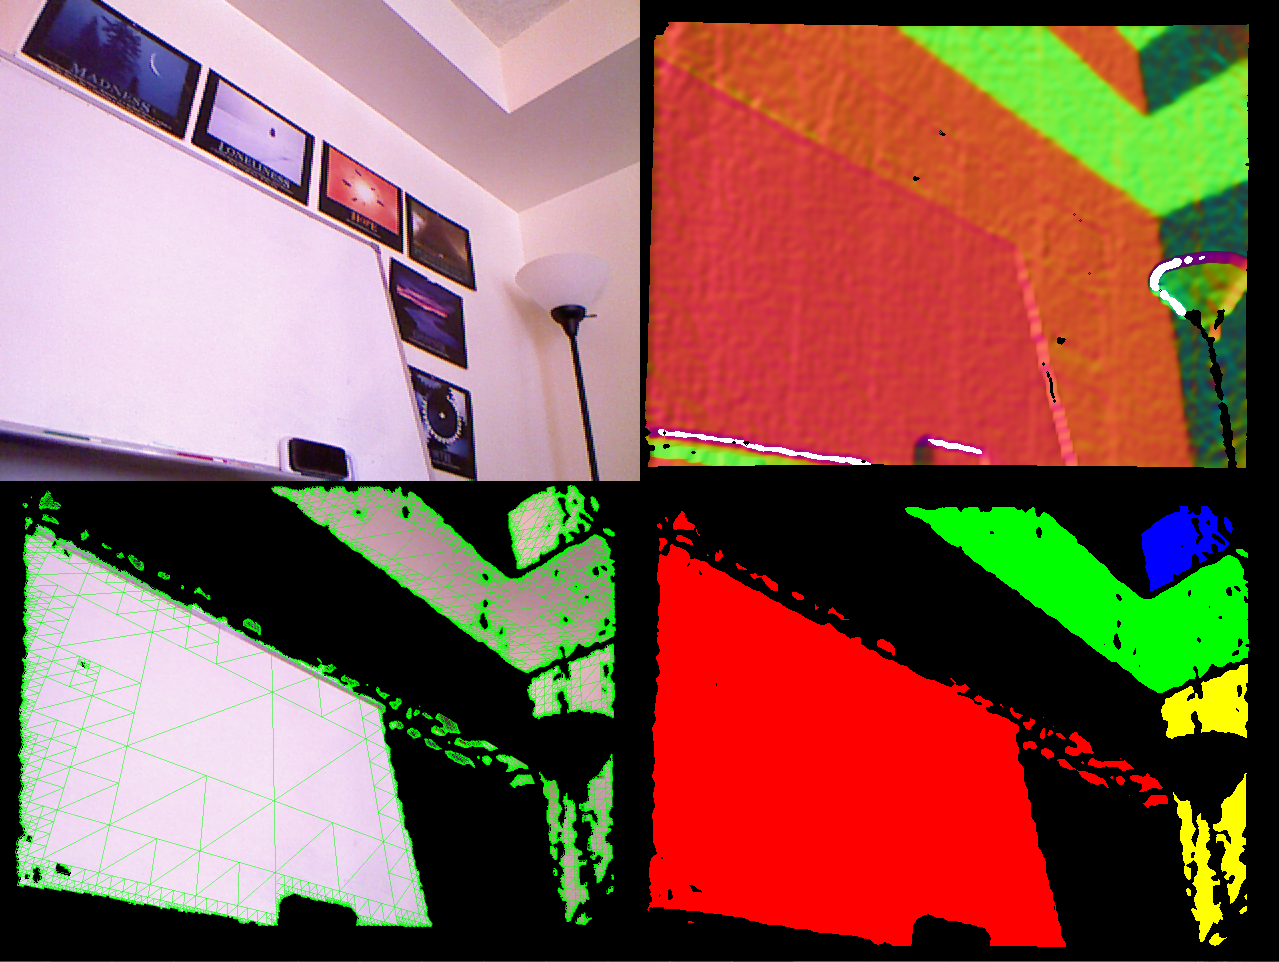
\includegraphics[width=0.8\textwidth]{MissingWall.png}
    \caption{Two planes with similar normals, only one is detected. Upper left) original color image. Upper right) surface normal estimates. Lower left) mesh reconstruction. Lower right) Random colorization of plane segments}
    \label{fig:missingwall}
\end{figure}



\begin{figure}[!htpb]
    \centering
    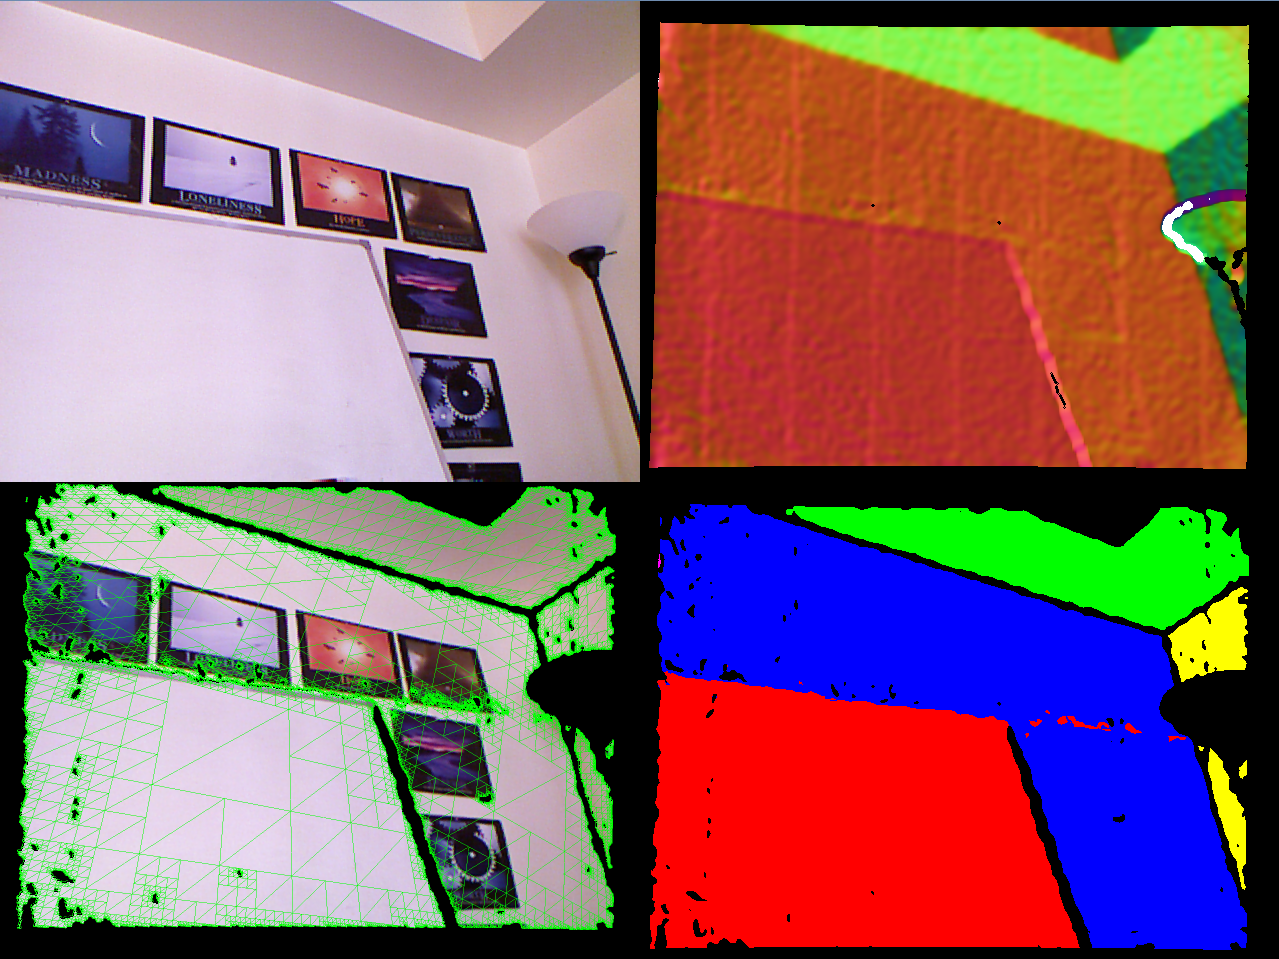
\includegraphics[width=0.8\textwidth]{PlaneIntersection.png}
    \caption{Two nearly parallel planes that intersect show some segmentation errors. Upper left) original color image. Upper right) surface normal estimates. Lower left) mesh reconstruction. Lower right) Random colorization of plane segments}
    \label{fig:planeintersect}
\end{figure}






\section{Performance Analysis}


\begin{figure}[!htpb]
    \centering
    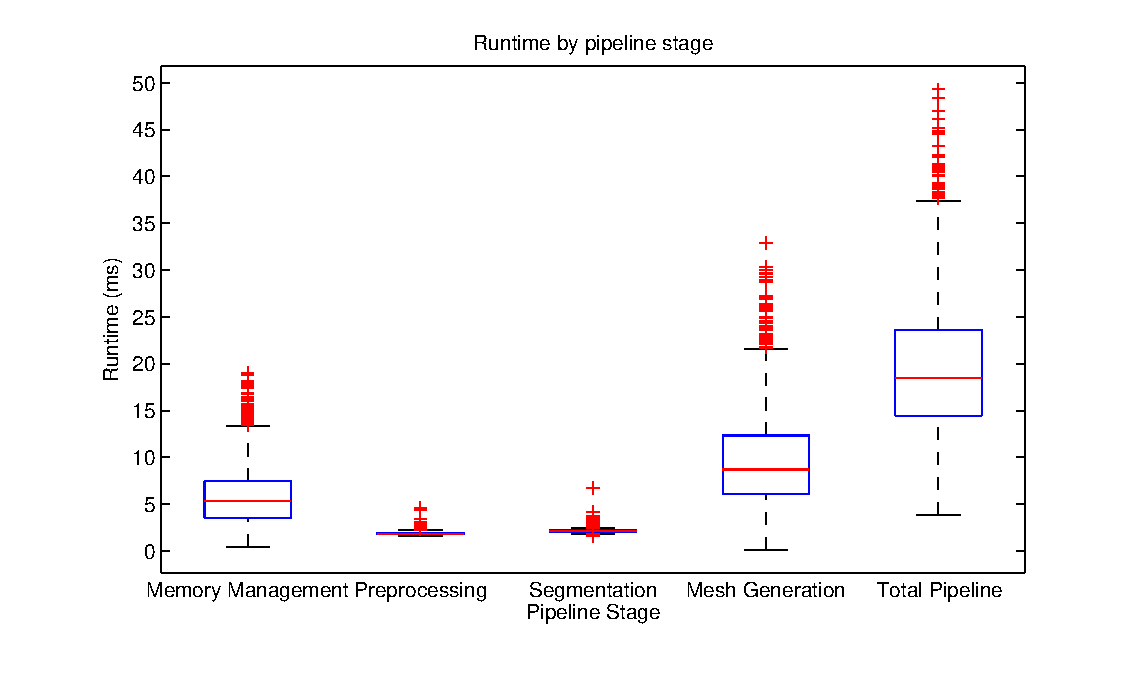
\includegraphics[width=1.0\textwidth]{RuntimeByPipelineStage.eps}
    \caption{Pipeline runtime broken down by stage.}
    \label{fig:runtimebystage}
\end{figure}

\begin{figure}[!htpb]
    \centering
    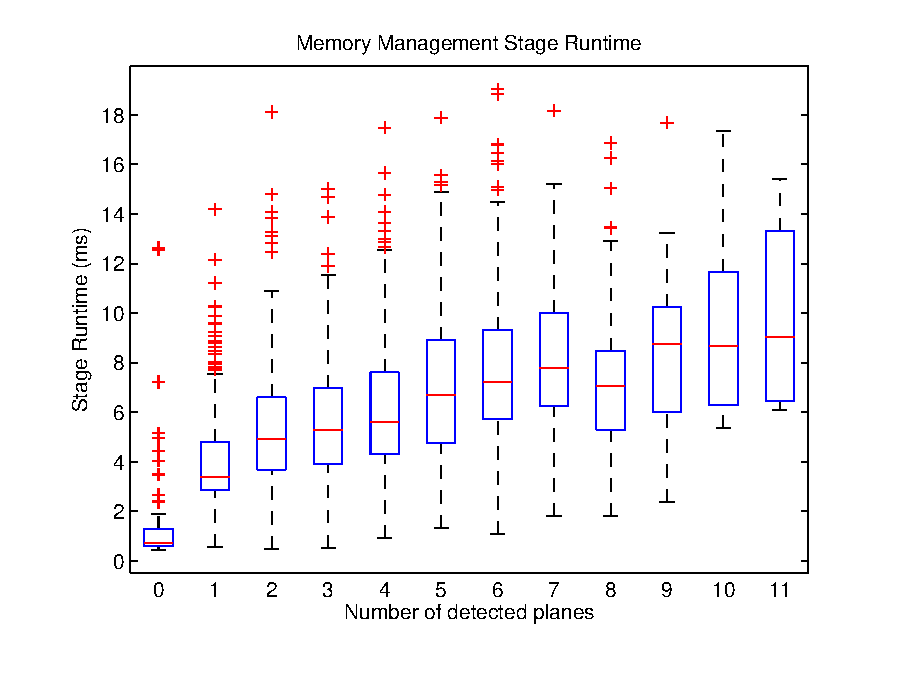
\includegraphics[width=0.7\textwidth]{MemoryManagementByNumPlanes.eps}
    \caption{Runtime of the memory management stage by number of detected planes.}
    \label{fig:memorymangementplanes}
\end{figure}


\begin{figure}[!htpb]
    \centering
    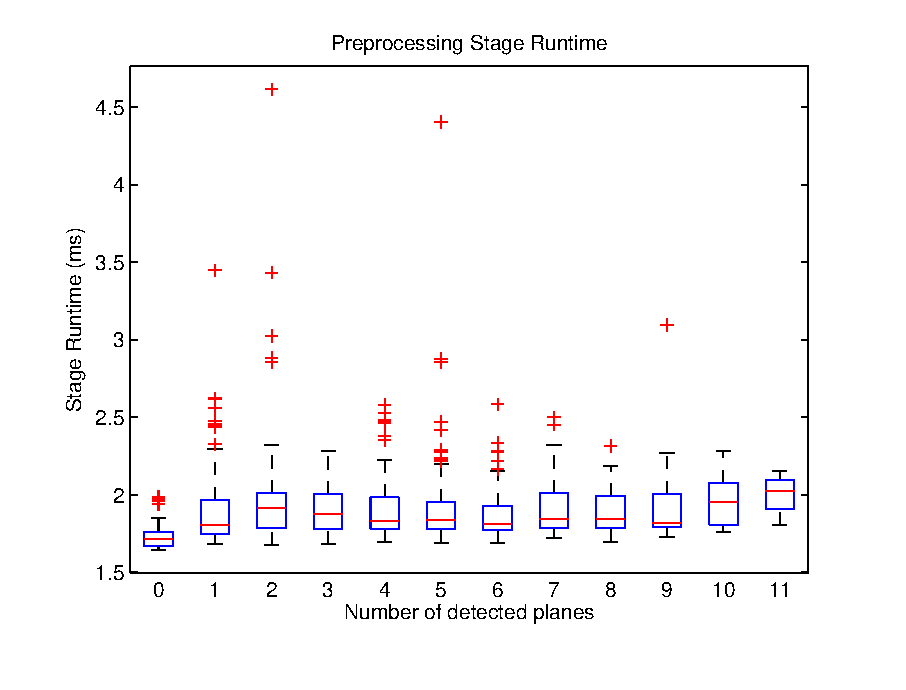
\includegraphics[width=0.7\textwidth]{PreprocessingByNumPlanes.eps}
    \caption{Runtime of the preprocessing stage by number of detected planes.}
    \label{fig:preprocessingplanes}
\end{figure}



\begin{figure}[!htpb]
    \centering
    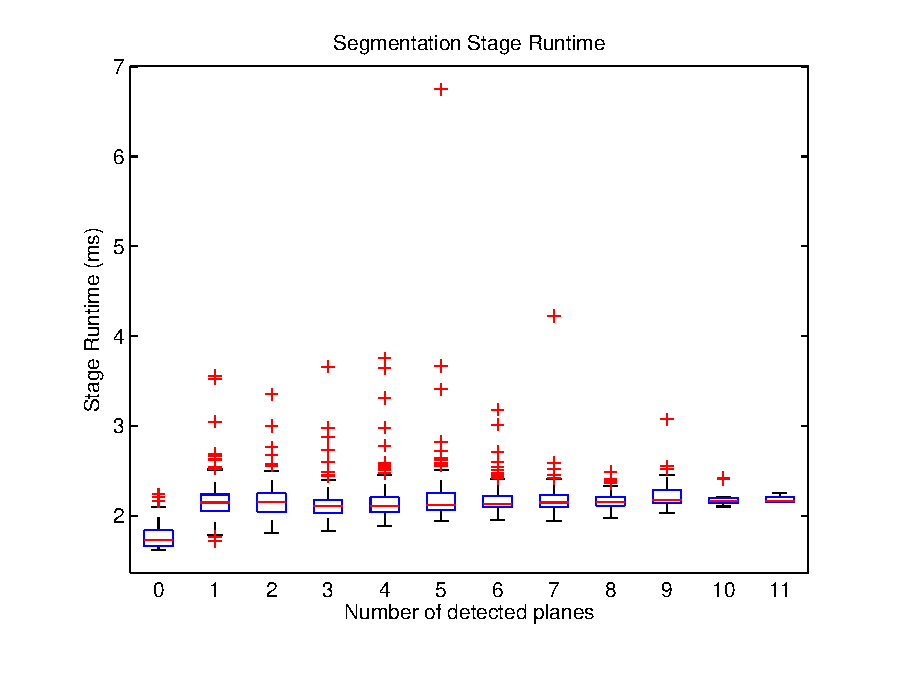
\includegraphics[width=0.7\textwidth]{SegmentationByNumPlanes.eps}
    \caption{Runtime of the segmentation stage by number of detected planes.}
    \label{fig:segementationplanes}
\end{figure}



\begin{figure}[!htpb]
    \centering
    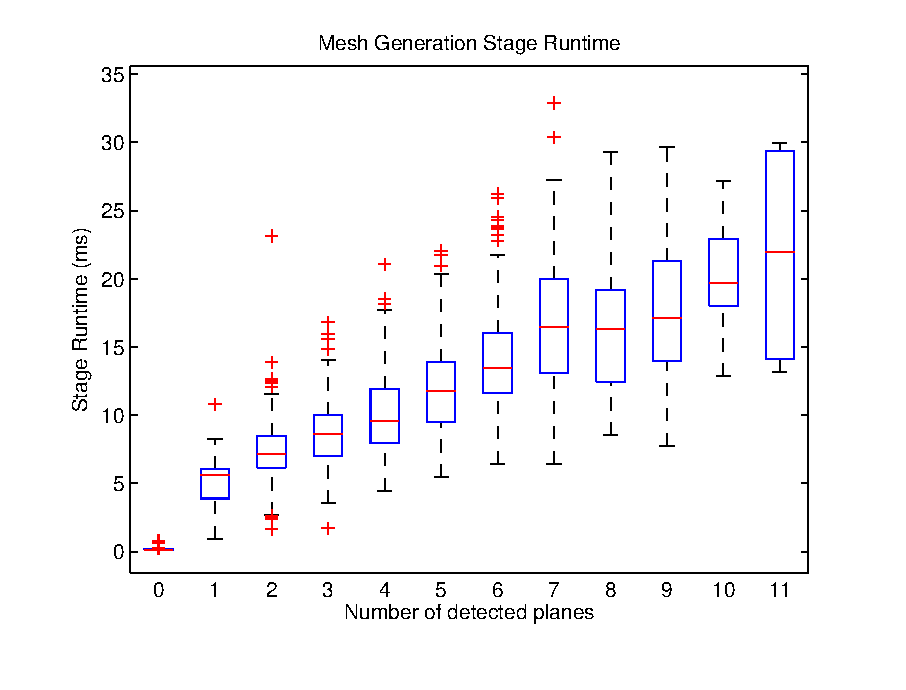
\includegraphics[width=0.7\textwidth]{MeshGenerationByNumPlanes.eps}
    \caption{Runtime of the mesh generation stage by number of detected planes.}
    \label{fig:meshgenerationplanes}
\end{figure}



\begin{figure}[!htpb]
    \centering
    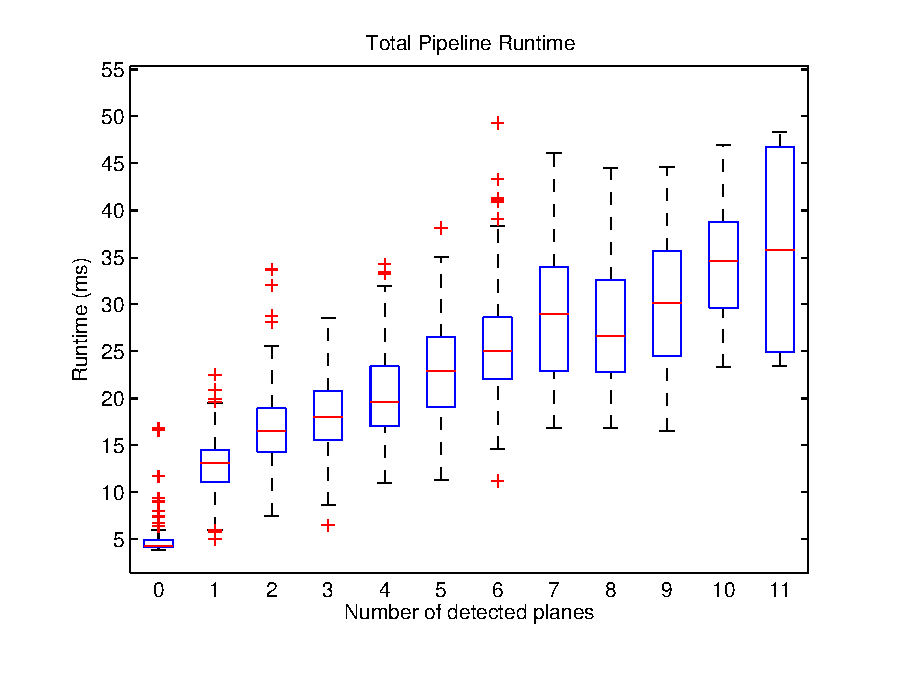
\includegraphics[width=0.7\textwidth]{PipelineByNumPlanes.eps}
    \caption{Runtime of the entire pipeline by number of detected planes.}
    \label{fig:pipelineplanes}
\end{figure}


